\section{Тест}
\subsection{Условие задания}
Создать приложение для проведения тестирования.

Должно содержать:

\begin{enumerate}
\item Набор вопросов по какой-то теме (и вопросы и ответы должны быть реальные) --- не менее 10
\item Вопросы должны выбираться случайным образом.
\item Вопросы должны быть нескольких типов - "Да/нет", Выбор одного ответа, Выбор нескольких ответов, Короткий ответ.
\item Необходимо создать сообщения для правильного и неправильного ответа (Молодец, Не правильно и т.д.)
\item Необходимо подсчитать количество правильных ответов и вывести результат.
\end{enumerate}

\subsection{Вид формы в конструкторе}
Форма имеет вид как на рисунке \ref{fig:test-form}

\begin{figure}
\centering
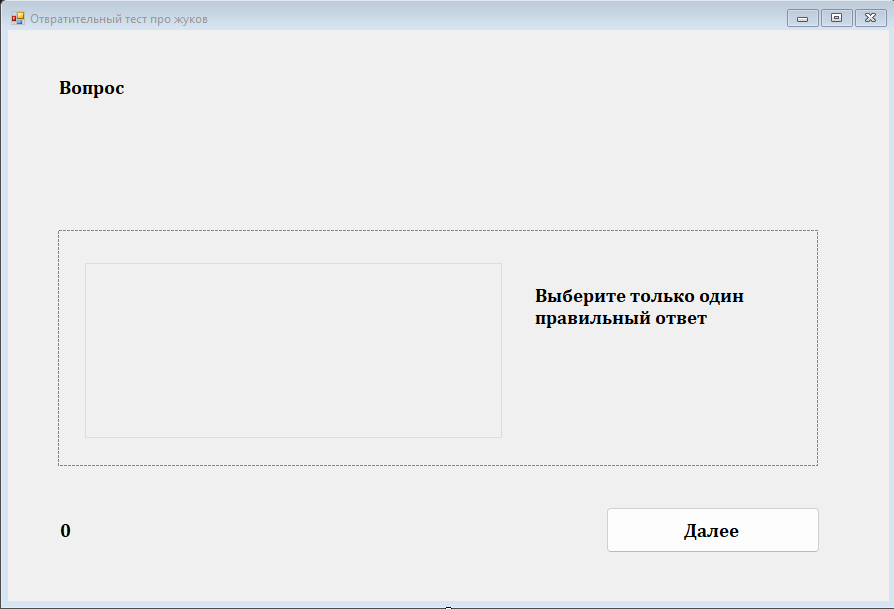
\includegraphics[width=0.5\linewidth]{images/test/form.png}
\caption{Форма окна для задания}
\label{fig:test-form}
\end{figure}

\subsection{Таблица с описанием элементов формы}
Все элементы формы были переименованы для большей читаемости. В таблице \ref{tab:test-form} представлены все изменения.


\begin{xltabular}{\textwidth}{| m{0.3\textwidth} | m{0.3\textwidth} | m{0.3\textwidth} |}

\hline
\textbf{Описание элементов формы} & \textbf{Список изменённых атрибутов} & \textbf{Новое значение атрибута} \\
\hline
\endfirsthead

\hline
\textbf{Описание элементов формы} & \textbf{Список изменённых атрибутов} & \textbf{Новое значение атрибута} \\
\hline
\endhead

\hline
\endfoot

\hline
\caption{Значение атрибутов элементов в приложении для работы с коллекциями}
\label{tab:test-form}
\endlastfoot

Окно формы & Text & Отвратительный тест про жуков \\
Динамическая метка для вопроса & Name & questionLabel \\

Панель\cite{panel} для единственного выбора ответа & Name & radioPanel \\
Группа\cite{group} для радиокнопок & Name & radioGroup \\
Метка для описания вопроса & Name & motivationRadioLabel \\

Панель для множественного выбора ответов & Name & checkPanel \\
Группа для множественного выбора & Name & checkGroup \\
Метка для описания вопроса & Name & motivationCheckLabel \\

Панель для ответа-строки & Name & textPanel \\
Группа для ответа-строки & Name & textGroup \\
Поле для ввода ответа-строки & Name & answerTextbox \\
Метка для описания вопроса & Name & motivationInputLabel \\

Метка для прогресса & Name & progressLabel \\
Кнопка для продолжения & Name & nextButton \\
\end{xltabular}

Все элементы добавляются из текущего вопроса динамически, также динамически происходит смена панели на нужную.

\subsection{Примеры правильной и неправильной работы приложения}
При запуске приложения на экране появляется окно \ref{fig:test-start}.

\begin{figure}
\centering
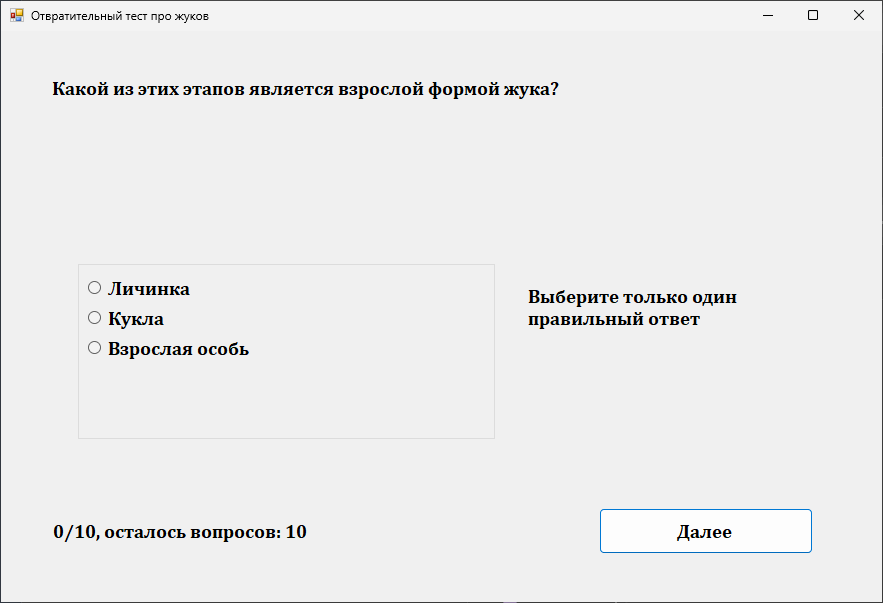
\includegraphics[width=0.5\linewidth]{images//test/start.png}
\caption{Запуск программы}
\label{fig:test-start}
\end{figure}

При нажатии на кнопки всё обрабатывается корректно. Также происходит обработка ошибок.

\begin{figure}
\centering
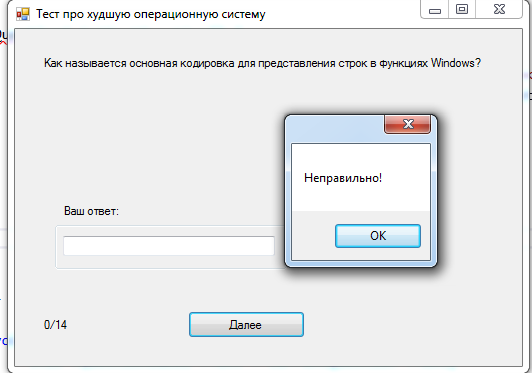
\includegraphics[width=0.5\linewidth]{images//test/okay.png}
\caption{Запуск с корректными данными}
\label{fig:test-okay}
\end{figure}

\begin{figure}
\centering
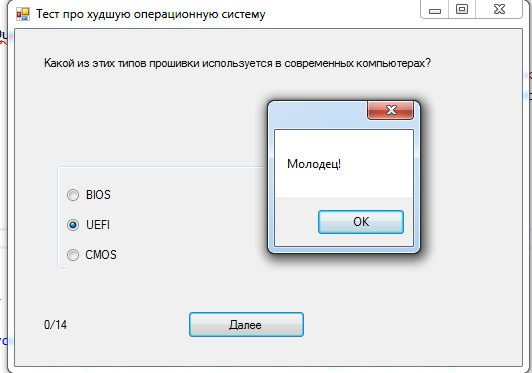
\includegraphics[width=0.5\linewidth]{images//test/okay2.png}
\caption{Запуск с корректными данными}
\label{fig:test-okay}
\end{figure}

\begin{figure}
\centering
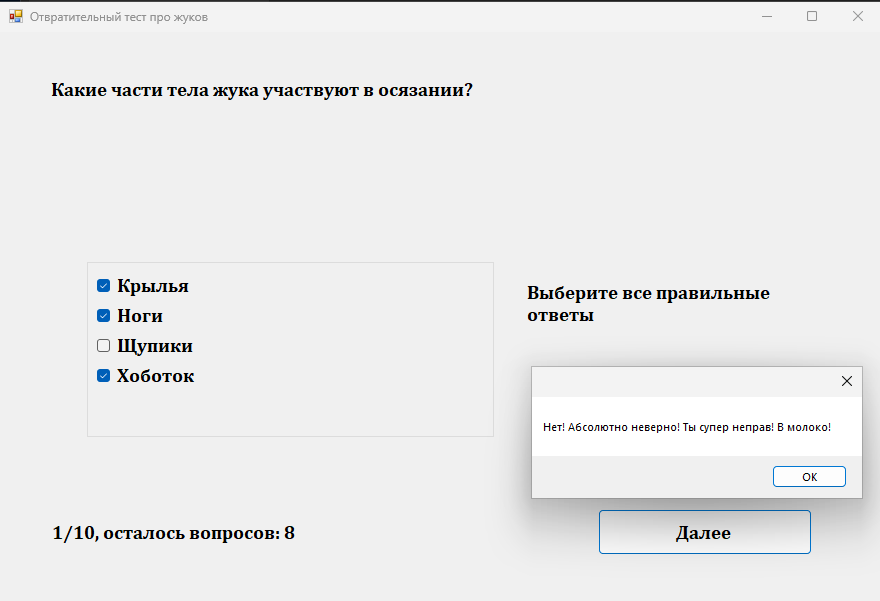
\includegraphics[width=0.5\linewidth]{images//test/okay3.png}
\caption{Запуск с корректными данными}
\label{fig:test-okay}
\end{figure}

\begin{figure}
\centering
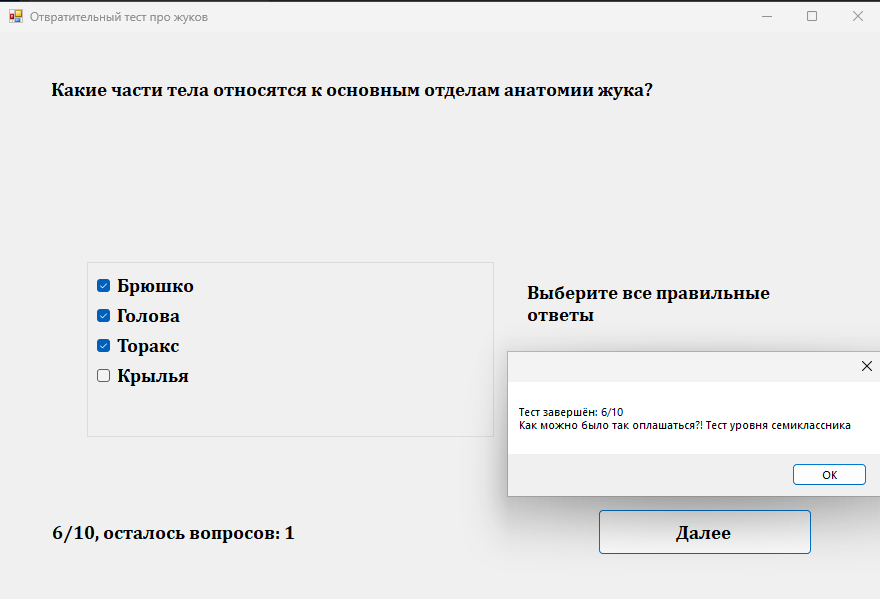
\includegraphics[width=0.5\linewidth]{images//test/okay4.png}
\caption{Пример ввода с некорректными данными}
\label{fig:test-error}
\end{figure}

Приложение спроектировано таким образом, что получить ошибку невозможно. При отсутствии ответа система его засчитает как неправильный, что вполне логично.

\subsection{Примеры исходного кода}
\begin{minted}{cpp}
	/// обновление результатов
	void UpdateResults() {
		this->progressLabel->Text = passed + "/" + total;
	}

	// активация радиовопроса
	void DisplayRadio() {
		this->radioGroup->Controls->Clear();
		radioPanel->Visible = true;
		checkPanel->Visible = false;
		textPanel->Visible = false;
	}

	/// активация множественного выбора
	void DisplayCheck() {
		checkGroup->Controls->Clear();
		radioPanel->Visible = false;
		checkPanel->Visible = true;
		textPanel->Visible = false;
	}

	/// активация строкового вопроса
	void DisplayText() {
		this->answerTextbox->Clear();
		radioPanel->Visible = false;
		checkPanel->Visible = false;
		textPanel->Visible = true;
	}
\end{minted}

Больше кода проекта доступно в приложении \ref{application-A}. Также в приложенном архиве можно найти полный код проекта.